\documentclass{beamer}
\usepackage{graphicx} % Required for including images
\usepackage{babel} % Required for language settings
\usepackage{listings} % Required for code listings
\usepackage{ragged2e} % Required for text justification
\usepackage{caption}
\captionsetup[figure]{name=}
\usefonttheme{professionalfonts}
\usetheme{metropolis}
\usecolortheme{orchid}
\title{ACHIEVO}
\subtitle{A Productivity WebApp}
\institute[Program]{
        \inst{Women Engineers}
        \inst{TalentSprint}
}
\date{17/09/2023}

\begin{document}

\begin{frame}
  \maketitle
\end{frame}

\begin{frame}{Team Members}
    \begin{itemize}
        \item Nidhi Iyer
        \item Khyati Satija
        \item Pankhuri Asthana
        \item Srinayana Mandalapu
        \item Anushka Shankar
    \end{itemize}
\end{frame}

\begin{frame}{Introduction}
    \begin{itemize}
        \item A user-centric web application for enhancing productivity.
        \item Addresses procrastination, lack of focus, and planning issues.
        \item Has features like Pomodoro, To-Do , Eisenhower matrix, etc.
    \end{itemize}
\end{frame}

\begin{frame}{Objectives}
    \begin{itemize}
        \item To learn web development via the process
        \item To implement our learnings and knowledge into our web-app.
        \item To deploy it and provide a solution to the raised issue.
    \end{itemize}
\end{frame}

% \begin{frame}{Approach}
%     \begin{itemize}
%         \item Collaborative Work.
%         \item User-Centric Design.
%         \item Frontend-First.
%         \item Backend Development.
%         \item Iterative Development.
%     \end{itemize}
% \end{frame}

\begin{frame}{Tech Stack}
    \begin{figure}
        \begin{minipage}[t]{0.2\textwidth}
            \centering
            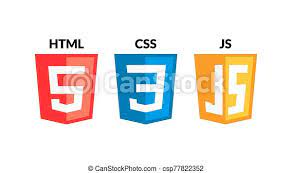
\includegraphics[width=\textwidth]{frontend.jpeg}
            \caption{Frontend}
        \end{minipage}\hfill
        \begin{minipage}[t]{0.2\textwidth}
            \centering
            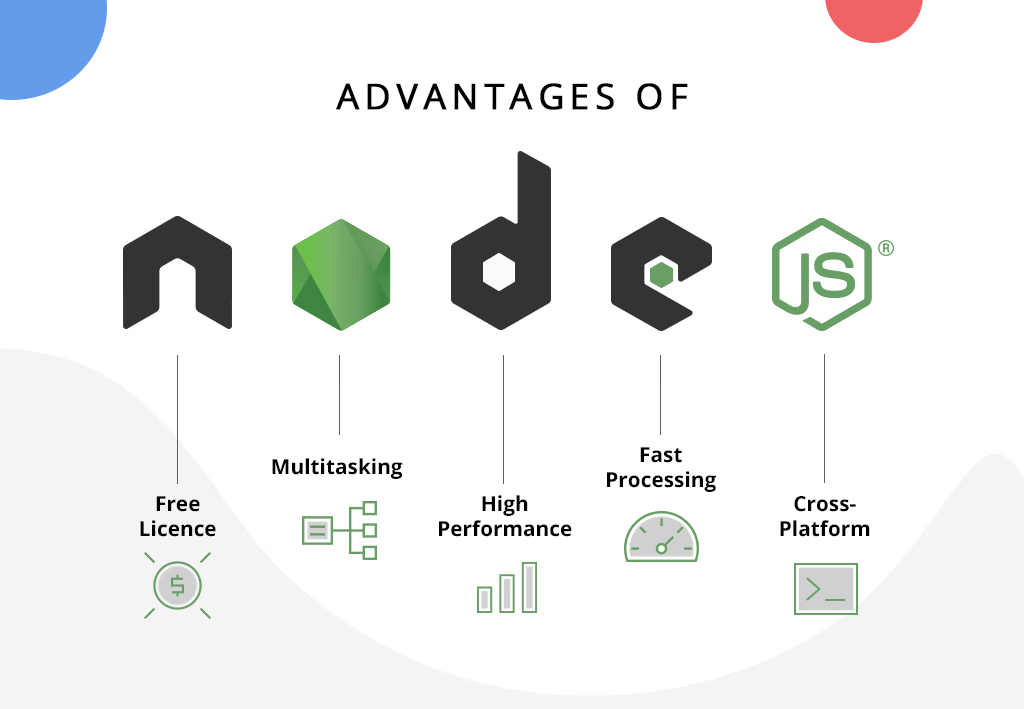
\includegraphics[width=\textwidth]{node.js_backend.png}
            \caption{Backend}
        \end{minipage}\hfill
        \begin{minipage}[t]{0.2\textwidth}
            \centering
            
\includegraphics[width=\textwidth]{mongoDB.png}
            \caption{Database}
        \end{minipage}\hfill
        \begin{minipage}[t]{0.2\textwidth}
            \centering
            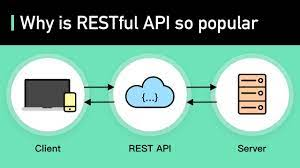
\includegraphics[width=\textwidth]{API.jpeg}
            \caption{RESTful APIs}
        \end{minipage}\hfill
    \end{figure}
\end{frame}

\begin{frame}{Project Details}
    \textbf{Work Done}
    \begin{enumerate}
        \item Started - 
        \item Paused  - 
        \item Resumed - 
    \end{enumerate}
    \textbf{GitLab Repository and Commit History}
    \bigskip
    \\
    \textbf{Code statistics}
    \begin{table}
        \centering
        \begin{tabular}{cc}
        \hline
        Language & Lines Of Codes \\
        \hline
        HTML & 500 \\
        CSS & 600 \\
        Javascript & 300 \\
        NodeJS & 600 \\
        EspressJS & 200 \\
        MySQL & 400 \\
        \hline
        \end{tabular}
        % \caption{A Simple Two-Column Table}
    \end{table}
\end{frame}      

\begin{frame}{Challenges and Learnings}
    \textbf{Challenges}
    \begin{enumerate}
        \item Inconsistent with the project
        \item Lacking in time management
        \item Taking excess time for backend
    \end{enumerate}
    \textbf{Learnings}
    \begin{enumerate}
        \item Team collaboration and project management
        \item Learnt MERN Stack technologies
        \item Breaking things down into smaller parts makes implementation easy.
    \end{enumerate}
\end{frame}

\begin{frame}{Future Scope}
  \begin{itemize}
    \item Good Scroll.
    \item Points for Pomodoro.
    \item Leaderboard.
    \item Marathon Mode.
    \item Fill the Container.
    \item The Hour Rule.
  \end{itemize}
\end{frame}

\begin{frame}{Conclusion}
    \justifying
    \centering
    Hence, Let's ACHIEVO \\
    \bigskip
    \bigskip
    \centering
    \Huge\textbf{Thank You !}
\end{frame}

\end{document}

